\section{The Plane and the Sphere}
\label{sec:plane-sphere}


The sphere and the plane are two surfaces that we will
frequently encounter. 
Stereographic projection, shown in \figref{stereo1}, is a map between almost all of the sphere
and the plane.
In order to gain intuition we first consider the one dimensional version of stereographic
projection between almost all of the circle and the real line.

\begin{example}[Stereographic Projection \cite{christian-notes}]\label{ex:stereo}
Consider the two sphere with the north pole removed $\Sp^2 \setminus (0,0,1)$,
stereographic projection is a bijection between the points on $\Sp^2 \setminus (0,0,1)$ to the $\R^2$.
Consider a line from the north pole $(0,0,1)$ that intersects $(x,y,z)\in \Sp^2$ parametrized by 
$p(t)=(1-t)(0,0,1)+t(x,y,z)$. By considering the $z$ coordinate we determine the $t$ value where this line
intersects $\R^2$, namely $t=\frac{1}{1-z}.$
This gives the desired map shown in  and in equation form
$$p(x,y,z)\to \left(\frac{x}{1-z},\frac{y}{1-z}\right).$$
\end{example}

\begin{figure}[htb]
	\centering
	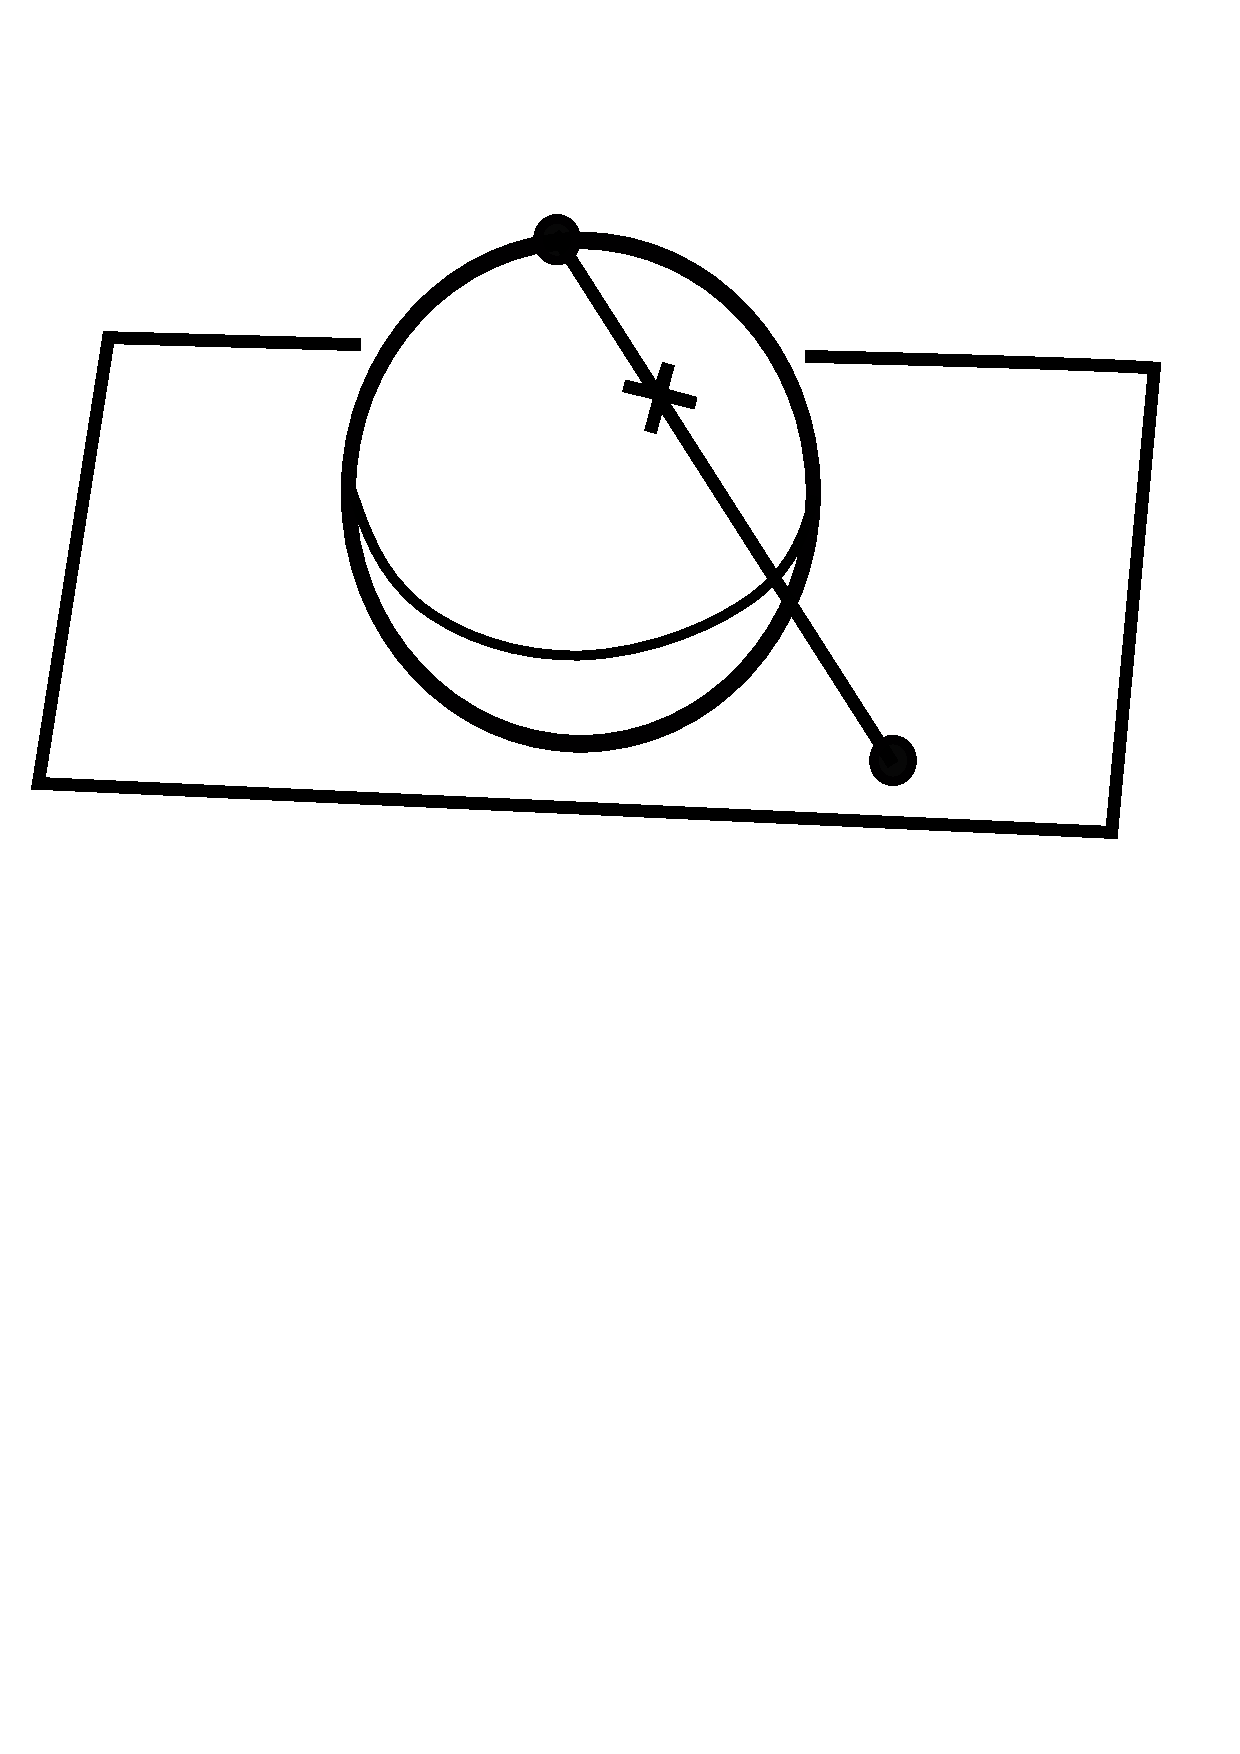
\includegraphics[width=.3\textwidth]{curvature/stereo}
	\caption{A point on the sphere is mapped to a point on the plane by stereographic projection.}
	\label{fig:stereo1}
\end{figure}
	
